\lab{Algorithm}{Kruskal's and Prim's Algorithm}{Kruskal's and Prim's Algorithm}
\label{Ch:Kruskal}

\objective{Find a minimum spanning tree for a connected weighted graph using Kruskal's Algorithm and Prim's Algorithm.}

\section*{Weight Graphs and Spanning trees}

Remember that a graph is composed of two sets: a set of nodes and a set of edges that connect these nodes. 

\begin{figure}[H]
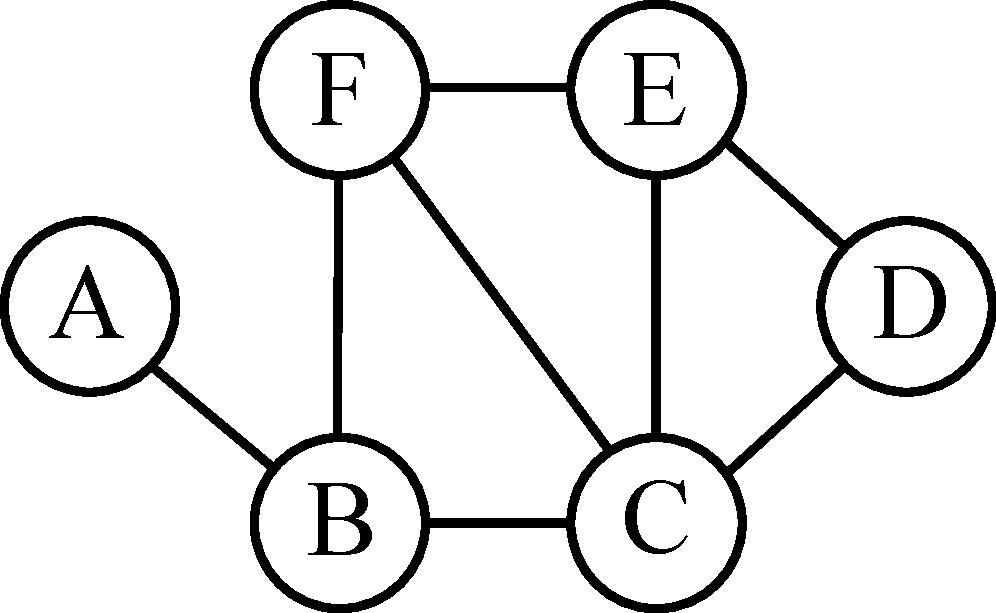
\includegraphics[width = .4\textwidth]{graph1.pdf}
\caption{An example of a graph}
\label{mst:graph1}
\end{figure}

A graph is directed if connections are uni-directional, and undirected if they are bi-directional.
Figure \ref{mst:graph1} shows an undirected graph.
A weighted graph is a graph where each edge has a value associated with it.
Usually these values represent some sort of cost or distance.
A connected graph is a graph where there is a path,or a set of edges, that connect every two nodes together.
We can write a matrix that describes this type of graph.
We let each row of our matrix represent a starting point and each column represent a destination.
If a path from one node to another exists, we put the weight of the path.
If there is no path, we put a 0.
For the above graph we generate the following matrix:

\[
A = \begin{pmatrix}
0 & 1 & 0 & 0 & 0 & 0\\
1 & 0 & 1 & 0 & 0 & 1\\
0 & 1 & 0 & 1 & 1 & 1\\
0 & 0 & 1 & 0 & 1 & 0\\
0 & 0 & 1 & 1 & 0 & 1\\
0 & 1 & 1 & 0 & 1 & 0\\
\end{pmatrix}
\]

This matrix is called an adjacency matrix.
Note that this matrix is symmetric, since the graph is undirected. 

Another way to store the graph is as a list of the edges and their weights that are connected (for an unweighted graph you can just store the edges).
It would look like this:

\[
[('A', 'B'),
 ('B', 'C'),
 ('B', 'E'),
 ('B', 'F'),
 ('C', 'D'),
 ('C', 'E'),
 ('C', 'F'),
 ('D', 'E'),
 ('E', 'F')]
\]

A third entry would store the wieght.

For this lab, we will be forcusing on undirected weighted graphs. 

A spanning tree of a connected undirected graph $G$ is is an undirected graph that contains all the nodes of $G$, a subset of the edges, and no cycles.
A cycle, for undirected graphs, is a path where you start and end on the same node without crossing any edge more than once.
Figure \ref{mst:graph3} shows a cycle in an undirected graph.

\begin{figure}[H]
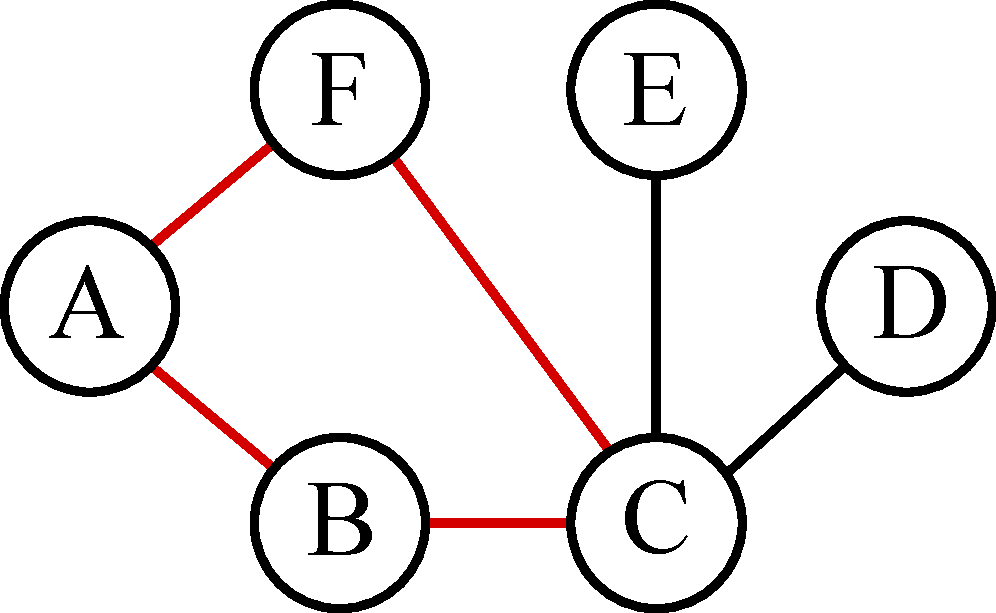
\includegraphics[width = .4\textwidth]{graph3.pdf}
\caption{A cycle in an undirected graph}
\label{mst:graph3}
\end{figure}

The minimum spanning tree (MST) of a wieghted, undirected graph is a spanning tree where the sum of the weights of the subset of edges is less than or equal to the sum of the weights of every other spanning tree.
Both Kruskal's and Prim's Algorithms are methods that find the minimum spanning tree of a weighted directed graph.
Figure \ref{mst:graph2} shows a minimum spanning tree of the graph shown in \ref{mst:graph1}.

\begin{figure}[H]
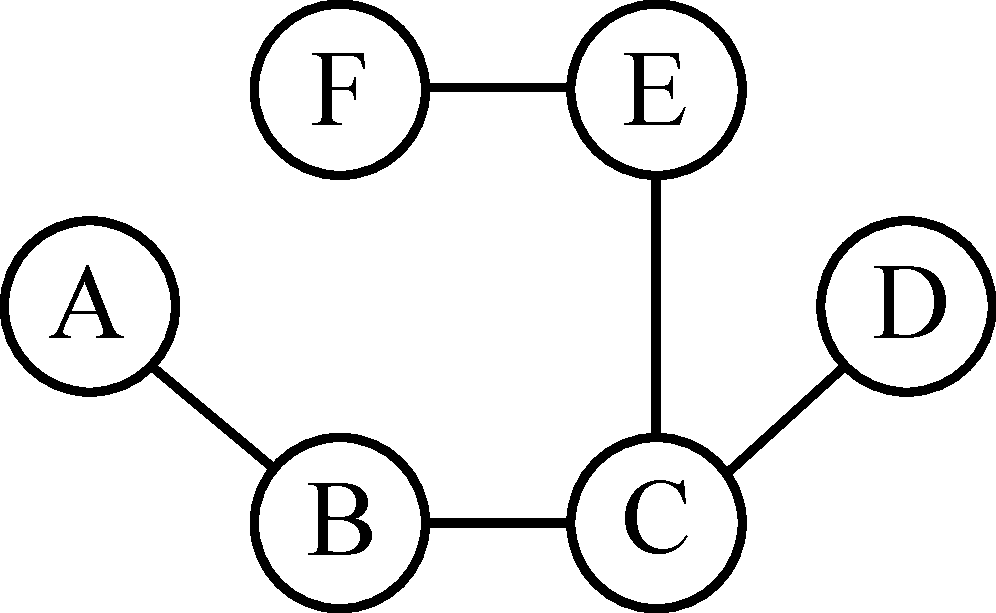
\includegraphics[width = .4\textwidth]{graph2.pdf}
\caption{An example of an minimum spaning tree for the previous graph}
\label{mst:graph2}
\end{figure}

\begin{figure}[H]
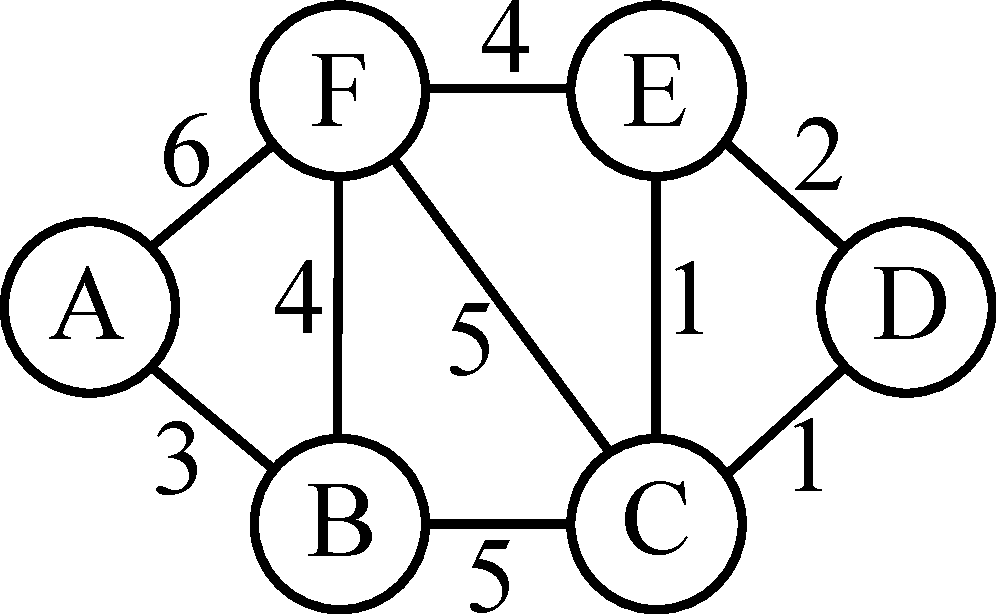
\includegraphics[width = .4\textwidth]{graph4.pdf}
\caption{A weighted directed graph}
\label{mst:graph4}
\end{figure}

\begin{figure}[H]
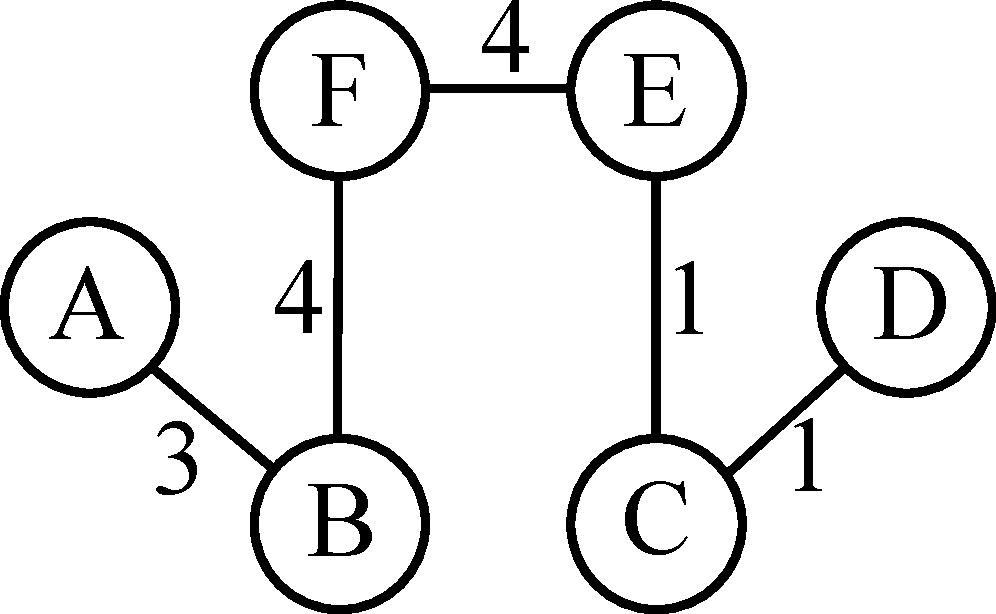
\includegraphics[width = .4\textwidth]{graph5.pdf}
\caption{The MST of the graph in Figure \ref{mst:graph4}.}
\end{figure}

\section*{Kruskal's algorithm}

Given a weighted directed graph G with $n$ nodes, Kruskal's algorithm finds the minimum by: first sorting the edges from smallest to largest.
Then, starting from the smallest, the alogrithm adds the edge to the tree as long as the addition of the new edge does not create a cycle.
When $n-1$ edges have been added, the algorithm stops.
% (put in an example)
In other words, given a weighted undirected graph G with $n$ nodes, Kruskal's algorithm finds the minimum spanning tree by sorting the edges from smallest to largest.
The fastest way to do this is as follows:

\begin{itemize}

% Revise the algorithm description. Especially the bit about pointers.

\item Sort the edges by weight in descending order.

\item Initialize pointers to trees

\item For each edge $e=\{x, y\}$, until $n-1$ edges added  

\begin{itemize}

\item if $x$ and $y$ are not in the same tree (i.e. don’t have the same root), add $e$

\item merge smaller tree (of $x$ or $y$) into larger tree 

\end{itemize}

\end{itemize}

\begin{problem}
Write Kruskal's algorithm.
Test your algorithm on random symmetric matrices.
Use the graph above and the data from MSTdata.npy to test your tree.
Use np.load("MSTdata.npy") to get it.
Use the formChanger function to put it in the right form.
% describe what formChanger does
\end{problem}

\section*{Prim's algorithm}

Prim's algorithm accomplishes the same thing as Kruskal's algorithm, but it uses a different approach.
Starting from any node it adds the edge with the least weight.
Those two nodes form a tree.
It than adds edges with the least weight to any node in the tree to any node not in the tree until all the nodes have been added.
The fastest way to do this is as follows:

\begin{itemize}

% Revise algorithm description

\item Start with the smallest-weight edge $e = \{x, y\}$ in $S$

\begin{itemize}

\item discard $x$ and $y$ from the list of nodes to consider

\item for both $x$ and $y$, find the closest node, if any (among the non-discarded nodes), and keep them and their edge weights

\end{itemize}

\item Until $n-1$ edges have been added

\begin{itemize}

\item Find the edge $e = \{x, y\}$ such that:

\begin{itemize}

\item $x$ is in $S$ and $y$ is not in $S$

\item $e$ is the smallest weighted edge left

\end{itemize}

\item add $e$ and $y$ to $S$

\item discard y from the list of nodes to consider, and for both $x$ and $y$, find the closest node, if any (among the non-discarded nodes), and keep them and their edge weights

\end{itemize}

\end{itemize}

\begin{problem}
Write Prim's algorithm.
Test your implementation with the same data as the previous problem.
Compare the speed of Prim's algorithm with Kruskal's algorithm. 
\end{problem}

\section*{Complexity}

Let $n$ be the number of nodes and $m$ be the number of edges.
Kruskal's Algorithm is O($m\log{n}$) which in the worst case is O($n^2\log{n}$).
Prims's Algorithm is O($n^2$).
So when the adjacent martix is sparse Kruskal's is better and when it is dense Prim's is better. 